
% This LaTeX was auto-generated from an M-file by MATLAB.
% To make changes, update the M-file and republish this document.

\documentclass{article}
\usepackage{graphicx}
\usepackage{color}

\sloppy
\definecolor{lightgray}{gray}{0.5}
\setlength{\parindent}{0pt}

\begin{document}

    
    
\subsection*{Contents}

\begin{itemize}
\setlength{\itemsep}{-1ex}
   \item Ejercicio 5 - Aprendizaje basado en redes y algoritmos clásicos
   \item Ejercicio 5.1
   \item Ejercicio 5.2
   \item perceptron.m
   \item Ejercicio 5.3
   \item kmedias.m
   \item Ejercicio 5.4
   \item redfuncbaserad.m
   \item funcbr.m
   \item Ejercicio 5.5
   \item kvecinos.m
   \item Ejercicio 5.6.
   \item ANALIZAR EN EL TEX
\end{itemize}


\subsection*{Ejercicio 5 - Aprendizaje basado en redes y algoritmos clásicos}

\begin{verbatim}
clc; clear all; close all;
\end{verbatim}


\subsection*{Ejercicio 5.1}

\begin{par}
Genere un conjunto de datos aleatorios bidimensionales separados en dos clases gaussianas correlacionadas con cierto grado de solapamiento.
\end{par} \vspace{1em}
\begin{verbatim}
N = 200; % cantidad de muestras

mu1 = [1 2];                % media clase 1 (+)
sigma1 = [0.9 0.3; 0.3 1.7];  % covarianza clase 1 (+)
mu2 = [4 4];                  % media clase 2 (o)
sigma2 = [1.5 -0.7; -0.7  3]; % covarianza clase 2 (o)

x1 = mvnrnd(mu1, sigma1, N); % ejemplos de la clase 1 (+)
x2 = mvnrnd(mu2, sigma2, N); % ejemplos de la clase 2 (o)
eti1 = ones(N,1);            % etiquetas de los ejemplos de la clase 1 (+)
eti2 = (-1)*ones(N,1);       % etiquetas de los ejemplos de la clase 2 (o)

% Graficacion de las distribuciones
hold on
plot(x1(:,1), x1(:,2),'+b')
plot(x2(:,1), x2(:,2),'or')
legend('clase 1','clase 2')
title('Distribuciones de los patrones')
xlabel('x_1'); ylabel('x_2');
axis equal
hold off

% Separacion entre entrenamiento y testeo, a utilizar cuando corresponda
nentre = floor(0.7 * N); % 70% de los patrones para entrenamiento
ntest = N - nentre;      % 30% de los patronespara testeo

% ejemplos de entrenamiento
xentre = vertcat(x1(1:nentre,:), x2(1:nentre,:));
% etiquetas para entrenamiento supervisado
etientre = vertcat(eti1(1:nentre), eti2(1:nentre));
% ejemplos de testeo
xtest = vertcat(x1(nentre+1:end,:), x2(nentre+1:end,:));
% etiquetas para testeo
etitest = vertcat(eti1(nentre+1:end), eti2(nentre+1:end));

% Ordeno de forma aleatoria los ejemplos de entrenamiento
ordenentre = randperm(2*nentre);
xentre = xentre(ordenentre,:);
etientre = etientre(ordenentre);
\end{verbatim}

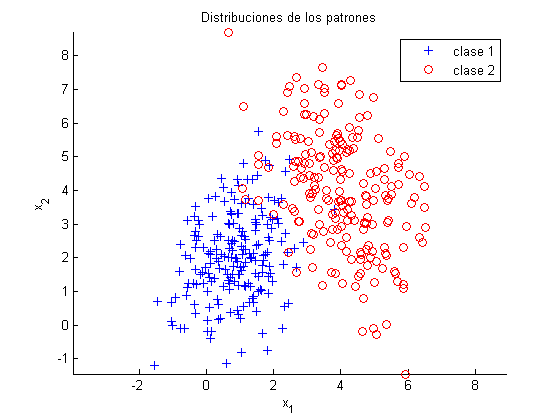
\includegraphics [width=4in]{Ejercicio5_01.png}


\subsection*{Ejercicio 5.2}

\begin{par}
Implemente el algoritmo de entrenamiento de un perceptron simple y pruebelo con los datos anteriores, grafique los resultados obtenidos.
\end{par} \vspace{1em}


\subsection*{perceptron.m}

\begin{verbatim}
dbtype perceptron.m

aprendizaje = 0.001; % coeficiente de aprendizaje
toler = 0.01;        % error tolerado en el entrenamiento
% entrenamiento
w = perceptron(xentre,etientre,aprendizaje,toler);
% testeo
etipercep = sign([ones(2*ntest,1) xtest] * w');

x1test = xtest(etipercep == eti1(1),:);%patrones identificados como clase 1
x2test = xtest(etipercep == eti2(1),:);%patrones identificados como clase 2

figure
hold on
plot(x1test(:,1), x1test(:,2),'+b')
plot(x2test(:,1), x2test(:,2),'or')
plot(xtest(etipercep~=etitest,1), xtest(etipercep~=etitest,2),'.k')
plot([1.5 4],-(w(1)+w(2)*[1.5 4])./w(3),'k-')
legend('clase 1','clase 2','errores')
title('Clasificaci�n con Perceptron Simple')
xlabel('x_1'); ylabel('x_2');
axis equal
hold off

errorpercep = sum(etipercep~=etitest) / ntest;
\end{verbatim}

        \color{lightgray} \begin{verbatim}
1     function [w, y] = perceptron( X, yd, alfa, tolerancia, iterMax)
2     % [w, y] = perceptron( X, yd, alfa, tolerancia, iterMax) entrena un 
3     % perceptron a partir de los patrones X y sus clases conocidas yd.
4     %   X son las caracteristicas, cada ejemplo en un renglon
5     %   yd es la salida deseada, la clase de cada ejemplo
6     %   alfa el coeficiente de aprendizaje
7     %   tolerancia de error admitida durante el entrenamiento
8     %   w es el vector de pesos aprendidos, el primer elemento es del bias, w0
9     %   y es el resultado de la clasificaci�n de los patrones de entrenamiento 
10    if nargin < 3
11        alfa = 0.05; % coef de aprendizaje
12    end
13    if nargin < 4
14        tolerancia = 0.1; % tolerancia en el error de entrenamiento
15    end
16    if nargin < 5
17        iterMax = 100; % tolerancia en el error de entrenamiento
18    end
19    
20    N = size(X,1);          % cantidad de patrones de entrenamiento
21    nCarac = size(X,2);     % cantidad de caracteristicas
22    
23    Xbias = [ones(N,1), X]; % agrego unos para entrenar bias
24    y = zeros(size(yd));    % clasificacion de los patrones de entrenamiento
25    
26    w = 0.5*rand(1,nCarac+1); % inicializo los pesos, incluido el del bias
27    error = 1;
28    iter = 0;
29    
30    while (error > tolerancia) && (iter < iterMax)
31        iter = iter + 1;
32        for n = 1:N
33            % salida del perceptron para el patron X(j)
34            y(n) = sign( dot( w, Xbias(n,:) ) );
35            w = w + alfa * (yd(n) - y(n)) * Xbias(n,:); % ajuste de w
36        end
37        error = norm(yd-y) / N;
38    end
39    
40    % Actualizo la clasificacion para los patrones de entrenamiento
41    y = sign(Xbias * w');
42    end
\end{verbatim} \color{black}
    
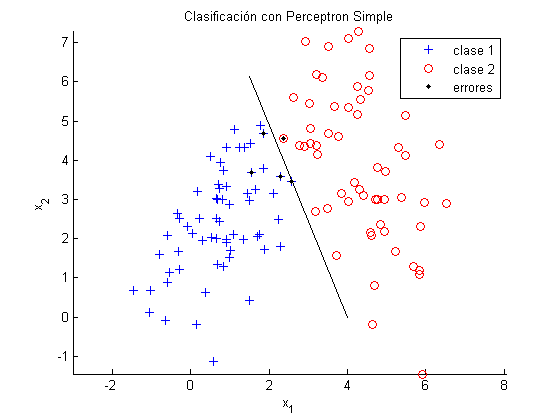
\includegraphics [width=4in]{Ejercicio5_02.png}


\subsection*{Ejercicio 5.3}

\begin{par}
Implemente el algoritmo de aprendizaje no supervisado k-medias (batch) y pruebelo con los datos anteriores, grafique los resultados obtenidos.
\end{par} \vspace{1em}


\subsection*{kmedias.m}

\begin{verbatim}
dbtype kmedias.m

[etikmed, med] = kmedias(xentre,2);

xAentre = xentre(etikmed == 1,:); %patrones asignados al grupo A
xBentre = xentre(etikmed == 2,:); %patrones asignados al grupo B

figure
hold on
plot(xAentre(:,1), xAentre(:,2),'xb')
plot(xBentre(:,1), xBentre(:,2),'dr')
plot(med(1,1),med(1,2),'*k')
plot(med(2,1),med(2,2),'*k')
legend('grupo A','grupo B','medias')
title('Agrupamiento con k-medias')
xlabel('x_1'); ylabel('x_2');
axis equal
hold off
\end{verbatim}

        \color{lightgray} \begin{verbatim}
1     function [y, med] = kmedias( X, k, tolerancia, iterMax)
2     %[y, med] = kmedias( X, k, tolerancia, iterMax) agrupa los patrones X en k
3     %grupos. Devuelve la media de los grupos en med y el grupo asignado a cada
4     %patron en y.
5     %   X contiene los patrones, uno en cada renglon
6     %   k define la cantidad de grupos a utilizar
7     %   y grupo asignado a cada patron
8     %   med media de cada grupo por renglon
9     %   tolerancia para definir la convergencia de las medias
10    %   iterMax limita los ciclos posibles para ajustar la media
11    if nargin < 3
12        tolerancia = 0.001; % tolerancia en la convergencia de las medias
13    end
14    if nargin < 4
15        iterMax = 100; % tolerancia en el error de entrenamiento
16    end
17    
18    N = size(X,1);          % cantidad de patrones
19    nCarac = size(X,2);     % cantidad de caracteristicas
20    med = zeros(k,nCarac);  % donde guardo las medias de los k grupos
21    y = zeros(N,1);         % grupo asignado a cada patron
22    grupo = cell(k,1);      % lista los patrones de cada grupo
23    
24    % inicializaci�n, asigno grupos al azar y en igual cantidad
25    indices = randperm(N); % orden arbitrario de los indices
26    Nini = floor(N/k); % cantidad de patrones en cada grupo
27    
28    iter = 0;
29    cambio = 100;
30    while (iter < iterMax) && cambio > tolerancia
31        iter = iter +1;
32        
33        % asignaci�n de grupos
34        if iter == 1
35            % en la iteraci�n inicial asigno arbitrariamente
36            for g = 1:k
37                if g == k
38                    grupo{g} = indices(1+Nini*(k-1):end);
39                else
40                    grupo{g} = indices(1+Nini*(g-1):Nini*g);
41                end
42            end
43        else
44            % en las restantes iteraciones asigno cada patron al centroide mas 
45            % cercano
46            grupo = cell(k,1); % olvido los grupos del paso previo
47            for n = 1:N
48                for g = 1:k
49                    distancias(g) = norm( X(n,:) - med(g,:) );
50                end
51                [~, gmin] = min(distancias);
52                grupo{gmin} = [grupo{gmin} n];
53            end
54        end
55        
56        % actualizaci�n de medias
57        medAnteriores = med; % reservo las medias anteriores
58        for g = 1:k
59            med(g,:) = mean(X(grupo{g},:),1); % nuevas medias
60            y(grupo{g})=g; % asignaciones de cada patron a cada grupo
61        end
62        cambio = norm(med - medAnteriores); % cambio de posici�n de las medias
63    end
64    
65    end
66    

\end{verbatim} \color{black}
    
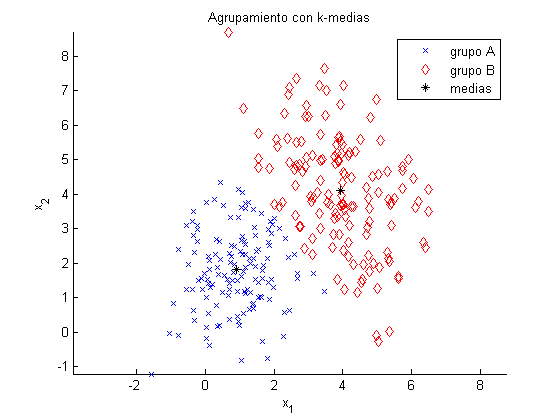
\includegraphics [width=4in]{Ejercicio5_03.png}


\subsection*{Ejercicio 5.4}

\begin{par}
Implemente el algoritmo de aprendizaje de las redes neuronales con funciones de base radial y pruebelo con los datos anteriores, grafique los resultados obtenidos.
\end{par} \vspace{1em}


\subsection*{redfuncbaserad.m}

\begin{verbatim}
dbtype redfuncbaserad.m
\end{verbatim}

        \color{lightgray} \begin{verbatim}
1     function [w, y, mu] = redfuncbaserad( X, yd, alfa, tolerancia, iterMax)
2     %[w, y] = redfuncbaserad( X, yd, alfa, tolerancia, iterMax) entrena una red
3     %neuronal con funciones de base radial.
4     %   X es una matriz de patrones donde cada uno se ubica en un renglon
5     %   yd es la salida deseada, la clase de cada ejemplo
6     %   alfa el coeficiente de aprendizaje
7     %   tolerancia de error admitida durante el entrenamiento
8     %   w es el vector de pesos aprendidos, el primer elemento es del bias, w0
9     %   y es el resultado de la clasificaci�n de los patrones de entrenamiento
10    %   la cantidad de funciones utilizadas es igual a la de clases presentes
11    %   en yd
12    if nargin < 3
13        alfa = 0.05; % coef de aprendizaje
14    end
15    if nargin < 4
16        tolerancia = 0.1; % tolerancia en el error de entrenamiento
17    end
18    if nargin < 5
19        iterMax = 100; % tolerancia en el error de entrenamiento
20    end
21    
22    N = size(X,1);       % cantidad de patrones de entrenamiento
23    nCarac = size(X,2);  % cantidad de caracteristicas
24    y = zeros(size(yd)); % clasificacion de los patrones de entrenamiento
25    
26    % inicializaci�n de las medias de las gaussianas con k-medias
27    k = length(unique(yd)); % k igual a la cantidad de clases
28    [~, mu] = kmedias(X,k); % utilizo las medias
29    
30    % considerando que las funciones de base radial son gaussianas con matriz
31    % de covarianza identidad, se definen como:
32    phi = @(xn,muj) exp(-0.5 * norm( xn-muj ).^2);
33    
34    % de cada patron obtengo nuevas caracter�sticas por medio de las gaussianas
35    Xnuevas = zeros(N,k); % nuevas caracteristicas
36    for n = 1:N
37        for j = 1:k
38            Xnuevas(n,j) = phi(X(n,:),mu(j,:));
39        end
40    end
41    
42    % ahora entreno un perceptron simple con las nuevas caracteristicas
43    w = perceptron(Xnuevas,yd,alfa,tolerancia,iterMax);
44    
45    % clasifico los patrones de entrenamiento
46    y = sign([ones(N,1) Xnuevas] * w');
47    
48    end
49    

\end{verbatim} \color{black}
    

\subsection*{funcbr.m}

\begin{verbatim}
dbtype funcbr.m

aprendizaje = 0.005; % coeficiente de aprendizaje
toler = 0.01;        % error tolerado en el entrenamiento
% entrenamiento
[w,~,mu] = redfuncbaserad(xentre,etientre,aprendizaje,toler);
% testeo
etirnfbr = sign([ones(2*ntest,1) funcbr(xtest,mu)] * w');

x1test = xtest(etirnfbr == eti1(1),:);%patrones identificados como clase 1
x2test = xtest(etirnfbr == eti2(1),:);%patrones identificados como clase 2

figure
hold on
plot(x1test(:,1), x1test(:,2),'+b')
plot(x2test(:,1), x2test(:,2),'or')
plot(xtest(etirnfbr~=etitest,1), xtest(etirnfbr~=etitest,2),'.k')
% plot([1 4],-(w(1)+w(2)*[1 4])./w(3),'k-')
legend('clase 1','clase 2','errores')
title('Clasificaci�n con Red Neuronal de Funciones de Base Radial')
xlabel('x_1'); ylabel('x_2');
axis equal
hold off

errorrnfbr = sum(etirnfbr~=etitest) / ntest;
\end{verbatim}

        \color{lightgray} \begin{verbatim}
1     function p = funcbr( X, mu )
2     % p(n,j)=fbr(X,mu)= exp(-0.5 * norm( xn-muj ).^2);
3     p = zeros(size(X,1),size(mu,1));
4     
5     phi = @(xn,muj) exp(-0.5 * norm( xn-muj ).^2);
6     for n = 1:size(X,1)
7         for j = 1:size(mu,1)
8             p(n,j) = phi(X(n,:),mu(j,:));
9         end
10    end
11    
12    end
\end{verbatim} \color{black}
    
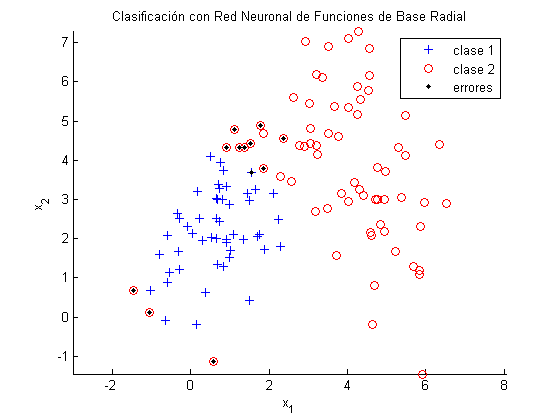
\includegraphics [width=4in]{Ejercicio5_04.png}


\subsection*{Ejercicio 5.5}

\begin{par}
5. Implemente el algoritmo de los k-vecinos m�s cercanos y pruebelo con los datos anteriores, grafique los resultados obtenidos.
\end{par} \vspace{1em}


\subsection*{kvecinos.m}

\begin{verbatim}
dbtype kvecinos.m

k = 10;
etikvec = kvecinos(xtest,k,xentre, etientre);

x1test = xtest(etikvec == eti1(1),:);
x2test = xtest(etikvec == eti2(1),:);

figure
hold on
plot(x1test(:,1), x1test(:,2),'+b')
plot(x2test(:,1), x2test(:,2),'or')
plot(xtest(etikvec~=etitest,1), xtest(etikvec~=etitest,2),'.k')
legend('clase 1','clase 2','errores')
title(['Clasificaci�n con k-vecinos m�s cercanos (k=' num2str(k) ')'])
xlabel('x_1'); ylabel('x_2');
axis equal
hold off

errorkvec = sum(etikvec~=etitest) / ntest;
\end{verbatim}

        \color{lightgray} \begin{verbatim}
1     function Cdesc = kvecinos( Xdesc, k, Xcon, Ccon )
2     %Cdesc = kvecinos( Xdesc, k, Xcon, Ccon ) clasifica los patrones
3     %desconocidos a partir de los k vecinos m�s cercanos conocidos.
4     %   Xdesc son los patrones a clasificar, cada uno en un renglon
5     %   k es la cantidad de vecinos a buscar para asignar la clase
6     %   Xcon son los patrones de clase conocida dada en Ccon
7     %   Xcon tiene cada patron por renglon, y cada elemento de Ccon est�
8     %   asociado al patr�n de Xcon que se ubicado en igual posici�n.
9     
10    Ndesc = size(Xdesc,1);  % cantidad de patrones desconocidos
11    Ncon = size(Xcon,1);    % cantidad de patrones conocidos
12    Cdesc = zeros(Ndesc,1); % clases asignadas a los patrones no vistos
13    
14    distancias = zeros(Ncon,1);
15    % A cada patron no visto le asigno su clase
16    for nd = 1:Ndesc
17        % Se calcula la distancia contra todos los conocidos
18        for nc = 1:Ncon
19            distancias(nc) = norm( Xcon(nc,:) - Xdesc(nd,:) );
20        end
21        
22        % se ordenan las distancias de menor a mayor
23        [~, orden] = sort(distancias); 
24        
25        % se listan las clases de los k vecinos mas cercanos
26        kvecclases = Ccon(orden(1:k)); % clases de cada uno de los k vecinos
27        clases = unique(kvecclases);    % clases posibles entre los k vecinos
28        cuenta = zeros(size(clases));  % cuantos patrones hay de cada clase?
29        for c = 1:length(clases)
30            cuenta(c) = sum(clases(c) == kvecclases);
31        end
32        [~, cmax] = max(cuenta); % clase con mayor presencia entre los k
33        
34        Cdesc(nd) = clases(cmax);% asignaci�n de clase al patron desconocido n
35    end
36    
37    end
38    

\end{verbatim} \color{black}
    
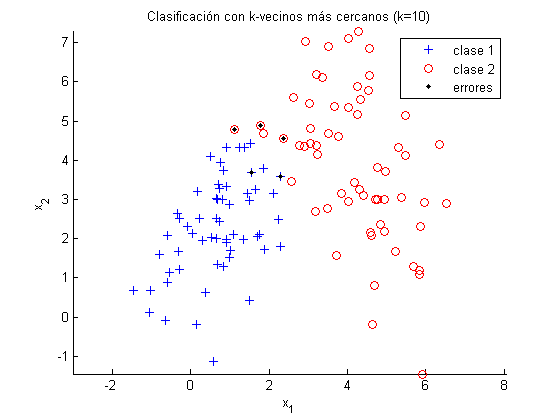
\includegraphics [width=4in]{Ejercicio5_05.png}


\subsection*{Ejercicio 5.6.}

\begin{par}
Compare y comente los resultados obtenidos por los distintos m�todos.
\end{par} \vspace{1em}
\begin{par}
Considerando los mismos grupos de testeo y entrenamiento los resultados durante el testeo fueron los siguientes:
\end{par} \vspace{1em}
\begin{verbatim}
fprintf('Tasa de error para el perceptron: %0.2f %%\n',100 * errorpercep);
fprintf('Tasa de error para la rn-fbr: %0.2f %%\n',100 * errorrnfbr);
fprintf('Tasa de error para el k-vecinos: %0.2f %%\n',100 * errorkvec);
\end{verbatim}

        \color{lightgray} \begin{verbatim}Tasa de error para el perceptron: 8.33 %
Tasa de error para la rn-fbr: 20.00 %
Tasa de error para el k-vecinos: 8.33 %
\end{verbatim} \color{black}
    

\subsection*{ANALIZAR EN EL TEX}




\end{document}
    
